\newcommand{\as}{\glqq}
\newcommand{\ad}{\grqq}
\newcommand{\adl}{\grqq{ }}

\newcommand{\fref}[1]{Abb. \ref{#1}} %Ref Figures

\section{Situationsanalyse} \label{sitana}
    In der Situationsanalyse beschäftigen wir uns mit der Mikro- und der Makroumwelt des Unternehmens. Dabei werden die 
    Persona betrachtet, welche wir als Musterkunden für unser Produkt angelegt haben. Auch haben wir uns die die 
    Branche, in welcher wir absetzen möchten, genauer angeschaut und hier eine Analyse der möglichen Absatzwege
    durchgeführt. Außerdem haben wir mittels der PEST-Analyse uns die generelle Situation unseres Standortes genauer
    angesehen. Mithilfe der SWOT-Analyse haben wir unsere Stärken, Schwächen, Chancen und Risiken noch einmal genauer 
    betrachtet.

    \subsection{Persona A} \label{personaA}
        Die erste Persona, welche wir uns überlegt haben, ist Clemens Müller. Clemens ist 70 Jahre alt. Er ist 
        verheiratet und hat Kinder, welche allerdings weit entfernt wohnen. Er hat in seinem Leben als Ingenieur
        gearbeitet, ist allerdings mittlerweile berentet. Seine hauptsächlichen Informationsquellen sind die Zeitung
        und das Fernsehen. In seiner Freizeit ist er Heimwerker oder bastelt an Eletronischen Geräten. 

        Er ein Interesse an unserem Produkt, da er sich eine körperliche Entlastung wünscht und selbstständiger sein
        möchte. In unserem Produkt such eine leichte Bedienbarkeit, eine lange Haltbarkeit und einen guten Service.

    \subsection{Persona B} \label{personaB}
        Bei unserer zweiten Persona handelt es sich um Andreas Martens. Andreas ist 40 Jahre alt, verheiratet und hat
        zwei Kinder. Er interressiert sich für unser Produkt, da er es sehr gut für seine Arbeit in der Gebäudepflege,
        welche er seit 20 Jahren ausübt, einsetzen kann. Außerdem ist er sehr Technikbegeistert und ist auf der Suche
        nach alternativen Arbeitswegen, mit welchen er sich seine Arbeit erleichtern und die Sicherheit erhöhen kann.
        Ebenfalls ist er auf der Suche nach mehr Effizienz und nach einem Zuverlässigen Produkt.

        Über neue technologische Entwicklungen informiert er sich vor allem über Fachmagazine, wie zum Beispiel \as Der
        Hausmeister\adl, oder auch über das Radio.

    \subsection{Branchenanalyse} \label{Branchen}
        Um die Situation und Position eines Unternehmens einordnen zu können steht u.a. die Branchenanalyse zur
        Verfügung. Bei der Branchenanalyse werden die Einflussfaktoren auf eine Branche ermittelt und bewertet. Dabei
        ist eine Branche ein Marktsegment mit Produkten, die untereinander substituierbar sind. Die Einflussfaktoren auf
        die Branche haben verschiedene Herkunft und auch unterschiedlich starken Einfluss.

        \noindent
        Das Five-Forces Modell nach Porter beschreibt die Einflussfaktoren, bewertet diese und stellt die
        Marktattraktivität da.

        \noindent
        Die Five-Forces (fünf Kräfte) bestehen aus der Verhandlungsmacht der Lieferanten (Vertragspartner bei denen
        Produkte eingekauft werden), der Verhandlungsmacht der Kunden, Bedrohung durch neue Wettbewerber 
        (Markteintrittsbarrieren), Bedrohung durch Ersatzprodukte (Substitute im weiteren Sinne) und der
        Wettbewerbsintensität der Branche. (Vgl. \cite{Gamayanto2005}, S.\,128-129)

        \noindent
        Die Verhandlungsmacht der Lieferanten beschreibt den Einfluss, den die Lieferanten auf das Unternehmen haben.
        Kann auf die Produkte des Lieferanten nicht verzichtet werden, sind z.B. keine Substitute vorhanden, wird das 
        Unternehmen abhängiger. Faktoren können die Anzahl der Anbieter, Vertragssicherheit, die Verzichtbarkeit und
        Substitute sein.

        \noindent
        Die Verhandlungsmacht des Kunden beschreibt den Einfluss der Kunden. Der Einfluss wächst mit zunehmender Anzahl
        an Marktbegleitern und Substituten. Wächst der Kundenkreis schneller als der Anbieterkreis (bei stetiger
        Produktionsmenge) sinkt die Verhandlungsmacht der Kunden. Sind die Umstellungskosten für die Kunden auf ein
        neues Produkt groß (Gewöhnung oder Verbundprodukte) sinkt auch der Einfluss.

        \noindent
        Bedrohung durch neue Wettbewerber. Hier stellt sich die Frage wie schwer es für potenzielle neue Anbieter ist
        den Markt zu betreten. Ist z.B. für die Herstellung eine bestimmte Genehmigung oder Handelspartner notwendig,
        sinkt das Risiko durch neue Wettbewerber. Sind die Einstiegsbarrieren aber niedrig, weil z.B. keine 
        kapitalintensiven Investitionen getätigt werden müssen, steigt das Risiko.

        \noindent
        Die Wettbewerbsintensität beschreibt die Gesamtsituation. Desto intensiver ein Wettbewerb ist, desto geringer
        sind die Aussichten auf ein gewinnbringendes Geschäft. Einflüsse wie Anzahl der Wettbewerber, Branchenwachstum,
        Austrittsbarrieren und Produktdifferenzierung spielen hier eine entscheidende Rolle. Anbieter, die keine starken
        Alleinstellungsmerkmale besitzen, können leichter aus der Branche gedrängt werden.

        %todo: Section anpassen
        \noindent
        Five Forces Modell angewandt

        \noindent
        Für die Verhandlungsmacht der Lieferanten wurde beispielhaft die Computer Chip Branche genutzt. Computer Chips
        werden von wenigen Produzenten in großer Stückzahl hergestellt. Dies Produzenten verkaufen große Mengen an
        Großhändler. Da die Menge an Chips pro Gerät vgl. gering ist, können viele Großhändler noch die extra
        Kapazitäten beim Hersteller einkaufen. Somit ist die Wahl des Großhändlers flexibel und der Lieferant hat eine
        geringe Verhandlungsmacht.

        \noindent
        Die Bedrohung durch neue Wettbewerber wird als gering betrachtet. Neue Wettbewerber müssen Kapital in der
        Entwicklung und den Aufbau einer Produktionsstätte binden. Zudem müssen für bestimmte Absatzwege hohe Barrieren
        überwunden werden (z.B. Aufnahme im Einzelhandel).

        \noindent
        Die Verhandlungsmacht der Kunden wird zur Markteinführung als gering eingeschätzt. Es wird davon ausgegangen,
        dass der Verkaufsstart auf einen ungesättigten Markt erfolgreich gelingt und die Nachfrage größer als das
        Angebot ist.

        \noindent
        Die Reinigung von Dachrinnen ist durch eine Vielzahl von Ersatzprodukten gekennzeichnet. So könnte der
        Hausbesitzer auf einen Dienstleister zurückgreifen oder die Dachrinnen eigenständig von Hand reinigen. Die
        Gefahr von Ersatzprodukten ist besonders im privaten Bereich groß.

        \noindent
        Aus den vier Bereichen kann die Rivalität unter den Wettbewerbern abgeleitet werden. Für die Erfolgsaussichten
        positiv ist die geringe Anzahl an Mitbewerbern, die geringe Macht der Lieferanten und Kunden und hohe
        Markteintrittsbarrieren.

        \noindent
        Negativ für die Erfolgsaussichten ist die Vielzahl an Ersatzprodukte, die finanziell günstiger und verbreiteter
        sind.

        \noindent
        Daraus lässt sich ableiten, dass die Rivalität auf dem Markt nicht sehr hoch ist und das Marktsegment große
        Erfolgsaussichten bieten. Für einen Erfolg sollte sich von Ersatzprodukten abgegrenzt werden.

        \begin{figure}[ht]
            \centering
            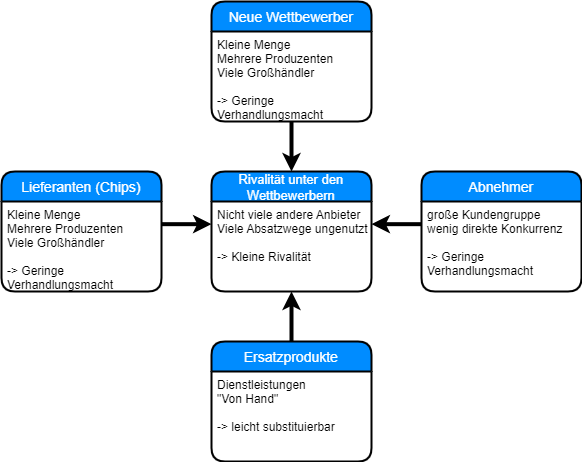
\includegraphics[width = 0.9\textwidth]{Eigene Darstellungen/Distributionswege2.png}

            \caption{Five Forces (Eigene Darstellung, in Anlehnung an \cite{Gamayanto2005}, S.\,127)}
        \end{figure}

\subsection{PEST-Analyse} \label{pest}
    Bei der PEST-Analyse bzw. der PEST(EL)-Methode um eine Überischtliche Darstellung der Makro-Umwelt des Unternehmens
    zu bekommen. Sie wurde im Jahr 1986 von Fahey und Narayanan entwickelt. Dabei werden die wesentlichen Rahmenfaktoren
    und Trends der globalen Unternehmensumwelt erfasst und 
    bewertet. Bei der Bewertung wird geschaut, welche Auswirkung die Faktoren der Makro-Umwelt auf das eigene 
    Unternehmen haben. Im folgenden werden einmal die einzelnen Teile der PEST-Methode erklärt und danach auf unser 
    Unternehmen bezogen.

        \begin{itemize}
            \item \textbf Political (Politisch)

                Hierbei handelt es sich die politische Situation des Landes in welchem das Unternehmen seinen Sitz hat 
                bzw. in welchem Land das Unternehmen produzieren oder verkaufen möchte. Dabei wird auf die Gesetzgebung 
                und auf die politischen Regulierungen geschaut und welche Auswirkungen diese auf zum Beispiel den Absatz
                des Unternehmens haben. Dazu zählt auch ob es für das geplante Produkt Regulierungen bezüglich der 
                legalität oder Absatzmengen einschränkungen gibt.

                Desweiteren wird die politische Stabilität des Landes in betracht gezogen. Denn auch diese kann 
                Auswirkungen auf die Entwicklung des Unternehmens haben. Bei einer Instabilen Lage kann es dazu kommen,
                dass sich das Unternehmen nicht am Markt halten kann und im schlimmsten Fall Insolvenz anmelden muss.

            \item \textbf Economical (Wirtschaftlich)
            
                Neben der politischen Lage ist auch die Wirtschaftliche Lage sehr wichtig für das Unternehmen. In diesem
                Teil der Analyse wird vorallem darauf geachtet, wie sich der Markt in der Region des Unternehmens bzw. 
                am Absatzort entwickelt. Es muss festgestellt werden ob ein gesättigter oder ungesättigter Markt 
                vorliegt und ob es für das Unternehmen möglich ist im gewünschten Markt Fuß zu fassen. Ein weiterer 
                wichtiger Faktor aus diesem Bereich sind die Steuerlichen Abgaben. Je nach höhe können diese ein 
                negativen Einfluss auf die Entwicklung des Unternehmens haben.

            \item \textbf Socio-Demographic (Sozio-Demographisch)
            
                Dieser Teil der Analyse befasst sich mit der Demographischen Situation. Wichtige Faktoren in diesem 
                Bereich sind zum Beispiel Trends oder das Kosumverhalten der Einwohner des Absatzlandes. Wenn zum 
                Beispiel die gewünschten Produktgruppe im gewünschten Absatzland nicht sehr beliebt ist und wenig 
                verkauft wird, sollte dies zu großen Teilen mit in die Entscheidung, ob an diesem Ort verkauft wird, 
                einfließen. Auch Ethnische und religöse Faktoren können hier in Betracht gezogen werden, wenn diese 
                Berührungspunkte mit dem abzusetzenden Produkt haben.

            \item \textbf Technological (Technologisch)
            
                Grade bei einem Unternehmen welches oft gute technologische Standards und deren Entwicklung angewiesen 
                ist, ist dieser Faktor sehr wichtig. Wenn ein Unternehmen zum Beispiel sehr viel über das Internet 
                arbeitet, also Online-Shops, Marketing etc., sollte sich dieses Unternehmen einen Standort aussuchen,
                welcher die nötige Infrastruktur bietet um das Konzept umzusetzen.

                Bei einem Unternehmen welche viel an der Forschung neuer Technologien arbeiten, wäre es hilfreich für 
                das Unternehmen wenn Forschung am möglichen Standort gefördert wird.
        \end{itemize}

    Beim Übertragen dieser Punkte auf das eigene Unternehmen sind wir zu folgenden Bewertungen unserers Standortes hier
    in Deutschland gekommen:

        \begin{itemize}
            \item Political
            
                Deutschland hat eine Politisch stabile Lage und gesetztlich gibt es wenige Regulierung. Auch der Export
                und Import sind durch die Europäische Union leicht möglich.

                Ein Thema welches allerdings in Deutschland immer mehr an Ansehen gewinnt, ist der Umweltschutz. Dies 
                führt dazu das wir bei unserer Produktion möglichst Umweltschonend vorgehen sollten, um das Ansehen des
                Unternehmens hier zu stärken und unserer Ziele  zu erreichen.

            \item Economical
            
                Deutschland hat eine insgesamt gute wirtschaftliche Situation. Durch aktuelle Ereignisse in der Welt 
                haben sich die Wechselkurse im Vergleich zu den Vorjahren verschlechter. Außerdem sind die steuerlichen 
                Abgaben hier in Deutschland vergleichweise hoch, was negative Auswirkungen auf unser Betriebsergebnis
                haben kann.

                Der Markt für einen Reinigungsroboter für Dachrinnen ist in Deutschland sehr klein, da es nur ein 
                anderes Konkurrzenprodukt gibt.
        \end{itemize}

\subsection{SWOT-Analyse} \label{swot}
Um nun externe und interne Informationsbereiche miteinander zu verbinden, wird die \as SWOT-Analyse\adl genutzt. Mit
dieser Betrachtung ist es möglich, die Stärken und Schwächen des Unternehmens kombiniert mit den Chancen und Risiken der
Mikro- und Makroumwelt zu untersuchen und Strategien abzuleiten.


\section{Marketing Mix} \label{Mix}


\subsection{Kommunikationspolitik} \label
    Nachdem nun die Produktpolitik betrachtet wurde, folgt die Kommunikationspolitik. Dieses Werkzeug des 
    Marketing-Mixes beschreibt die Wege, mit denen das Unternehmen mit seinen Kunden in Kontakt tritt und diese mit
    Informationen und Werbung versorgt. (Vgl. \cite{Kuss2016} S.\,203)

    \noindent
    Bei der Entwicklung der Kommunikationspolitik ist die Auswahl der Marketingträger und -plattformen von essenzieller
    Bedeutung. Um die wirkungsvollsten Träger auszuwählen, müssen zunächst wieder die Personas aus der Situationsanalyse
    betrachtet werden. Danach werden für diese Zielgruppen entsprechende Kommunikationswege gewählt.

    \noindent Im Fall \as RinnenRobo\adl gibt es die folgeden zwei Zielgruppen:

    \begin{enumerate}
        \item Hauseigentümer, vor allem ältere Personen
        \item Dienstleister in der Gebäudepflege
    \end{enumerate}

    \noindent Um für diese Zielgruppen nun die Kommunikationsmedien zu wählen, wird mit der Intermediaselektion begonnen.
    
    \noindent Für die erste Zielgruppe wurden folgende Medien herausgestellt:

        \begin{itemize}
            \item Fernsehen
            \item Radio
            \item Zeitung
        \end{itemize}

    \noindent Um die Dienstleister zu erreichen, wurden die folgenden Medien gewählt: 

        \begin{itemize}
            \item Fachmessen
            \item Fachmagazine
            \item Direktmarketing
        \end{itemize}

    \noindent
    Bei der Auswahl dieser Medien wurde betrachtet, auf welchen Medien die Personen der entsprechenden Zielgruppe häufig
    anzutreffen sind. Somit wären hier auch die Chancen für eine erfolgreiche Marketingkampagne hoch.

    \noindent
    Im nächsten Schritt werden die einzelnen Kommunikationskanäle genauer betrachtet und es findet die
    Intramediaselektion statt. Hierbei werden konkrete Möglichkeiten innerhalb der Plattformen herausgearbeitet. Dabei
    wird wieder versucht, die Teilkanäle zu wählen, bei denen ein Antreffen von potenziellen Kunden am
    wahrscheinlichsten ist.

    \noindent
    Die Intramediaselektion für die Gruppe der Hauseigentümer sieht folgendermaßen aus:

    \begin{itemize}
        \item Fernsehen
            \subitem Das Erste
            \subitem ZDF
            \subitem NDR
        \item Radio
            \subitem NDR 1
            \subitem Bremen 1
        \item Zeitung
            \subitem Lokale Tageszeitung
    \end{itemize}

    \noindent
    Für die Dienstleister wurden folgende Teilkanäle gewählt:

     \begin{itemize}
        \item Messen
            \subitem IPM Essen
            \subitem GaLaBau
            \subitem CMS Messe Berlin
        
        \item Fachmagazine
            \subitem Der Hausmeister
            \subitem Galabau Journal

        \item Direktmarketing
            \subitem Prospekte
            \subitem Flyer
     \end{itemize}

    \noindent
    Auf den genannten Teilkanälen wäre also eine Kommunikation mit Personen der entsprechenden Zielgruppe möglich.

    \noindent
    Um nun konkrete Marketingmaßnahmen planen und durchführen zu können, muss außerdem eine Budgetstrategie festgelegt
    werden. Diese Strategie besagt, wie viel Kapital für die Kommunikationspolitik ausgegeben werden darf. Dieses
    Kapital wird beispielsweise für Fernsehspots oder Werbeanzeigen in der lokalen Tageszeitung benötigt.
    (Vgl. \cite{Bruhn2014a}, S.\,212)

    \noindent
    Es gibt sowohl analytische als auch heuristische Verfahren zur Budgetierung. Bei den analytischen Ansätzen wird das
    verfügbare Kapital durch mathematische Funktionen errechnet, während dieses bei heuristischen Ansätzen nach
    vereinfachten Regeln festgelegt wird (vgl. \cite{Bruhn2014a}, S.\,214).

    \noindent
    Im Folgenden werden jedoch nur die heuristischen Ansätze weiter betrachtet.

    \noindent
    Diese heuristischen Verfahren lassen sich in drei weitere Untergruppen gliedern. Diese werden im Folgenden genannt
    und näher erläutert.

    \begin{itemize}
        \item Unternehmensbezogene Ansätze
            
            Bei dieser Art von Budgetierung werden unternehmensinterne Werte zur Budgetkalkulation herangezogen. So kann
            beispielsweise ein gewisser Prozentsatz des Umsatzes für Kommunikationsmaßnahmen eingesetzt werden.

        \item Konkurrenzbezogene Ansätze
        
            Hier orientiert sich ein Unternehmen an den Werbebudget und -ausgaben der Konkurrenz und versucht auf dessen
            Grundlage die eigene Marketingbudgetierung vorzunehmen.

        \item Marktbezogene Ansätze
        
            Bei diesen Ansätzen liegt der Fokus auf dem zu erreichenden Ziel. Daraus wird das benötigte Budget bestimmt.
            So kann das Ziel etwa eine Bekanntheit von 20\% auf dem deutschen Markt sein. Hieraus wird nun das zum
            Erreichen dieses Ziels benötigte Budget bestimmt.
    \end{itemize} (Vgl. \cite{Bruhn2014a}, S.\,214)

    \noindent
    Im Praxisbeispiel \as RinnenRobo\adl wird ein unternehmensbezogener Ansatz genutzt. Genauer: Es soll so viel
    Kapital für die Durchführung der Marketingmaßnahmen genutzt werden, wie verfügbar ist.

    \noindent
    Diese Entscheidung ist begründet durch das allgemeine Unwissen über die Existenz von Rinnenreinigungsrobotern und
    den Wunsch \as RinnenRobo\adl zu einer bekannten Marke zu entwickeln, um auch höhere Preise rechtfertigen zu
    können.



\subsection{Marketingziele}
    Marketingziele werden formuliert, um die Ressourcen in einem Betreib gemeinsam in eine Richtung einzusetzen. Dabei
    geben die Ziele bei Entscheidungen eine Orientierung und sollen die Mitarbeiter motivieren. Die Ziele müssen
    erreichbar sein, damit die Mitarbeiter nicht demotiviert werden. Ein wichtiger Aspekt der Ziele ist die
    anschließende Kontrolle der Zielerfüllung und Abweichungsanalyse, um ggf. neue Maßnahmen ableiten zu können. Diese
    Ziele sind mittel- bis langfristig ausgelegt. (Vgl. \cite{Becker2018}, S.\,60)

    \noindent
    Um die unterschiedlichen Aspekte und Vorgaben der Zielsetzung zu berücksichtigen kann die SMART-Methode angewandt
    werden Die SMART-Methode geht auf Peter Drucker zurück und bietet Kriterien zur eindeutigen Formulierung von
    überprüfbaren und umsetzbaren Zielen. Jeder Buchstabe von SMART beinhaltet ein Kriterium an die Zielformulierung.
    Werden alle Kriterien eingehalten, können Unternehmensziele formuliert werden. (Vgl. \cite{Lawlor2012}, S.\,269)

    \begin{itemize}
        \item Spezifisch
        
            Das Ziel muss eindeutig und konkret formuliert sein. Es dürfen keine Missverständnisse entstehen. Bsp.: 
            \as Der Umsatz ist in diesem Jahr gegenüber dem Vorjahr zu steigern.\ad

        \item Messbar

            Die Erreichung des Ziels muss messbar sein. So werden quantitative und qualitative Anforderungen an das Ziel
            gesetzt. Eine objektive Bewertung muss möglich sein. Bsp.: \as Der Umsatz ist in diesem Jahr gegenüber dem
            Vorjahr um 15\% zu steigern.\ad

        \item Attraktiv
        
            Die Zielsetzung muss für die Teammitglieder attraktiv und akzeptabel sein. Können die Mitglieder sich nicht
            mit dem Ziel identifizieren so sinkt die Motivation. So sollte z.B. eine gemeinnützige Unternehmung keine
            moralisch verwerflichen Ziele anstreben. 

        \item Realistisch
        
            Das Ziel muss realistisch und damit umsetzbar formuliert sein. Ist die Erreichung des Ziels unrealistisch
            sinkt die Motivation das Ziel zu erreichen. Werden Zwischenziele erreicht kann das die Motivation weiter
            antreiben.

        \item Terminiert
        
            Um das Erreichen der Ziele kontrollieren zu können muss ein Zeitpunkt zur Zielerfüllung festgelegt sein.
            Folglich ist das Ziel in einer bestimmten Zeit zu erreichen. Nachdem die Zeit abgelaufen ist, kann die
            Kontrolle und Abweichungsanalyse starten.
    \end{itemize}


    %TODO Section machen

    \noindent
    Die Marketingziele für den RinnenRobo

    \begin{enumerate}
        \item Ziel
        
            Der RinnenRobo soll innerhalb eines Jahres 25\% Bekanntheit auf dem deutschen Fachmarkt erreicht haben.

        \item Ziel
        
            Nach drei Jahren sollen 10.000 Einheiten auf dem deutschen Massenmarkt (Privat- und Geschäftskunden)
            abgesetzt worden sein.

        \item Ziel
        
            Auf dem europäischen Markt soll eine Bekanntheit von ca. 5\% erreicht werden. Das bedeutet jeder zwanzigste
            Europäer soll Berührungspunkte mit unserem Produkt gesammelt haben. Dazu zählt auch Werbung.
    \end{enumerate}


\section{Produktpolitik}
    Der Begriff Produktpolitik umfasst alle Entscheidungen, die sich auf die Gestaltung des Angebotes eines Unternehmen
    beziehen. Die Produktpolitik ist neben der Preispolitik, der Kommunikationspolitik und der Distributionspolitik ein
    Element im Marketing-Mix. Sie beschäftigt sich mit der Gestaltung des Produktes (Eigenschaften, Name, Verpackung),
    des Service (Beratung, Wartung) und des Sortiments (Angebote, Produktvariation). (Vgl. \cite{Bruhn2012}, S.\,28-29)

    \subsection{Ziele der Produktpolitik}
        Die Produktpolitik erfolgt zielorientiert, wobei verschiedene Ziele angestrebt werden.

        Ökonomische Ziele der Produktpolitik sind das Erzielen eines Gewinns, die Sicherstellung des Wachstums, die
        Optimierung der Wettbewerbsposition, die Minimierung des Risikos, eine möglichst hohe Kapazitätsauslastung sowie
        die Realisierung von Rationalisierungs- und Synergieeffekten.

        Psychologische Ziele der Produktpolitik ist die Steigerung des Goodwills (beispielsweise Firmenimage,
        Technologieführerschaft) sowie die positive Beeinflussung der Einstellung, mit der die Kaufinteressenten das
        Produkt beurteilen. (Vgl. \cite{Bruhn2012}, S.\,130)

    \subsection{Nutzenkomponenten eines Produkts}
        Ein Produkt ist ein Bündel von nutzenstiftenden Eigenschaften, dass die Befriedigung von Kundenbedürfnissen zum
        Ziel hat. Es wird zwischen zwei Nutzungsarten unterschieden.

        Grundnutzen: Mit dem Grundnutzen werden die grundlegenden Bedürfnisse eines Menschen befriedigt. Die Unternehmen
        nutzen den Grundnutzen, um Produkte herzustellen, die auf die Grundbedürfnisse abgestellt sind. Zu den
        Grundbedürfnissen zählen z. B. Wärme, Hunger und Mobilität.

        Zusatznutzen: Mit dem Zusatznutzen erfüllt das Produkt eines Unternehmens einen Nutzen, der über den Grundnutzen
        hinausgeht.

            \begin{itemize}
                \item Funktionaler Zusatznutzen
                
                    Über den Grundnutzen hinausgehende Bedürfnisbefriedigung durch das Produkt.

                \item Emotionaler Zusatznutzen
                
                    Aus den Emotionalen Wirkungen eines Produktes resultierende Bedürfnisbefriedigung.

                \item Sozialer Zusatznutzen
                
                    Aus den Sozialen Wirkungen eines Produktes resultierende Bedürfnisbefriedigung.
            \end{itemize}

        Im Fall \as RinnenRobo\adl hat das Produkt das Grundnutzen der Reinigung von Dachrinnen. Als Funktionaler
        Zusatznutzen kann zu dem Produkt eine Wetterstation installiert werden. Zudem wird die Inspektion des
        \as RinnenRobo\adl kostenfrei angeboten. 
            
        Der Emotionale Zusatznutzen gibt den Produktanwendern, in diesem Fall oftmals Personen der älteren Generation,
        ein Gefühl der Selbständigkeit, da sie unabhängig sind und keine persönliche Hilfe von anderen Personen erbitten
        müssen. 
        
        Der Soziale Zusatznutzen besteht darin, dass Anwender dieses Produktes Technisches Interesse zeigen. 
            
    \subsection{Produktvarianten}
        Ein Produkt kann in verschiedenen Varianten desselben Produkts verkauft werden, zum Beispiel in verschiedenen
        Farben und Größen. Wenn ein Produkt Varianten hat, heißt das übergeordnete Produkt, zu dem die Varianten
        erstellt werden, Hauptprodukt. Jede Variante kann einen eigenen Preis, eigene Bestandsinformationen,
        Produktinformationen usw. haben (Vgl. \cite{Bruhn2012}, S.\,131, 157).
        
        Das Produkt \as RinnenRobo\adl gibt es in zwei Hauptvarianten, für den privaten Anwender in drei Ausführungen
        und für die Unternehmer und Dienstleister in zwei Ausführungen.
            
        \subsubsection{RinnenRobo}
            \begin{itemize}
                \item RinnenRobo Light
                
                    Diese Variante ist günstiger als die beiden anderen. Sie hat nur eine Hauptaufgabe und zwar das
                    Reinigen der Dachrinne und keine zusätzlichen Features. 

                \item RinnenRobo Pro
                
                    Neben der Hauptaufgabe hat die Pro Variante alle zusätzlichen Features. Bei der Pro Variante kann
                    eine Wetterstation mit gebucht werden. Sie kann aktuelle Wetterdaten wiedergeben und mit dem
                    Smartphone können alle Funktionen abgerufen werden. Da sie alle Features enthält ist sie teuerste
                    Variante in der RinnenRobo Produktgruppe. 

                \item RinnenRobo Modular
                
                    Diese Variante hat unterschiedliche Preise, da beliebige Features neben der Hauptfunktion dazu
                    gewählt werden können. 
            \end{itemize}

        \subsubsection{RinnenRobo Business}
            \begin{itemize}
                \item RinnenRobo Rental
                
                    Da dieses Produkt teuer in der Anschaffung ist wird es von Dienstleistern erworben und diese bieten
                    es zum Mieten an.  

                \item RinnenRobo Smart
                
                    Diese Variante ist ähnlich wie die Pro Variante, ist aber für Unternehmen gedacht. Sie hat alle
                    Features und zusätzlich eine feste Ladestation. Die Unternehmen haben hier auch noch die Möglichkeit
                    ihr eigenes Firmenlogo auf den RinnenRobo aufzuzeichnen. 
            \end{itemize}

\subsection{Preisstrategie} \label{preisstrat}
    Bei der Wahl unserer Preisstrategie haben wir uns für die Premium-Strategie entschieden:
    
        \begin{itemize}
            \item Qualität
            
                Da wir in unserem Produkt eine hohe Qualität bieten, sind wir der Ansicht das wir für diese Produkt auch
                einen höher segmentierten Preis verlangen können.

            \item Image
            
                Durch ein stetig hohe Qualität wollen wir uns ein gutes Image aufbauen, in welchem unser Unternehmen für
                gute Qualität steht.

            \item Hohe Kosten

                Der Bau eines Roboters ist mit vielen Kosten verbunden. Ein sehr wichtiges Bauteil, das für alle Roboter
                benötigt wird, sind Chips. Doch in aktuellen Zeiten ist Chip-Industrie am Kapazitätslimit und die Preise
                sind hoch. Um diese Kosten stämmen zu können, müssen wir das Produkt im Premium Segment absetzen

            \item Made in Germany
            
                Unsere Produktion findet vollständig hier in Deutschland statt. Dadurch das wir hier produzieren, sind
                auch unsere Produktionskosten höher, was sich in unserem Preis wiederspiegelt. Allerdings steht \as Made
                in Germany\adl auch für eine gute Qualität und auch für gut Arbeitsbegingungen der Angestellten. Das
                hilft uns auch dabei ein gutes Image aufzubauen.

            \item Kundendienst
            
                Mit dem Kundendienst bieten wir eine zusätzliche Leistung über den eigentlichen Kauf des Produktes
                an. Damit diese zusätzlichen Kosten gedeckt werden können, muss der Preis auf einem höheren Niveau 
                angesetzt werden.

            \item Nischenmarkt
            
                Da es sich bei unserem Produkt um einen Nischenmarkt handelt, sind möglicherweise viele Menschen nicht 
                bereit das Geld für den \as RinnenRobo\adl auszugeben. Außerdem ist dies ein nicht sehr bekannter Markt.
                Um dieses Defizit kompensieren zu können haben wir uns für die Premium-Strategie entschieden.
        \end{itemize}

\subsection{Preisdifferenzierung} \label{Preisdiff}
    \begin{itemize}
        \item Zeitliche Strategie
            
        Bei der Zeitlichen Strategie haben wir uns für die Skimming-Strategie entschieden. Der Grund dafür ist, 
        wir grade zur Markteinführung einen höheren Absatz erwarten. 

        Ein weiterer Grund für diese Strategie ist, dass es sich um ein technisches Produkt handelt. In dieser
        Sparte wollen die meisten Menschen immer das neueste Produkt. Das bedeutet das sie nach einiger Zeit 
        nicht mehr bereit sind unseren Roboter zu einem sehr hohen Preis zu erwerben.

        \item Kundenbezogen

            Unser Unternehmen hat einen Unterschiedlichen Preis für Kunden aus dem B2B und dem B2C Bereich. Der Grund 
            hierfür liegt in unseren verschiedenen Produkten, welche wir einmal speziel für den B2C und den B2B Bereich
            Designed haben.

        \item Mengenbezogen
        
            Bei Bestellungen von großen Mengen bieten wir einen Mengenrabatt an. Wenn sich ein 
            Dienstleistungsunternehmen eine ganze Flotte Roboter kauft, hat dies für uns Kostentechnische Vorteile.
            Wir müssen das System bei dem Kunden nur einmal Einrichten und Erklären. Das bedeutet das wir bei einer 
            Bestellung von zum Beispiel 10 Robotern einen Ähnlichen Aufwand haben wie bei einer Bestellung von nur einem 
            Roboter.
        \end{itemize}

\subsection{Distributionspolitik} \label{distro}
    Distribution beschreibt die betriebliche Funktion zwischen Hersteller und Verbraucher. Damit beschreibt die
    Distributionspolitik alle Entscheidungen und Maßnahmen auf dem Weg vom Anbieter zum Konsumenten.

    \noindent
    Die Distributionspolitik ist ein maßgebendes Instrument wie an den Kunden herangetreten wird. Die
    Distributionsentscheidungen sind im Regelfall langfristig ausgelegt. Es müssen je nach Produkt komplexe
    Distributionsketten auf- und ausgebaut werden.

    \noindent
    Die Distributionspolitik verfolgt dabei Ökonomische-, Versorgungs- und Psychologische Ziele. Hauptbestandteil der
    Ökonomischen Ziele ist der Erhalt und Ausbau des Betriebs in dem z.B. neue Kundengruppen erschlossen werden. Die
    Versorgungsziele beschäftigen sich unter anderem mit Lieferzuverlässigkeit und Liefergeschwindigkeit. Der dritte
    Bereich, die Psychologischen Ziele beinhalten insbesondere das Auftreten und die Wahrnehmung des Unternehmens.
    (Vgl. \cite{Bruhn2014}, S.\,245-278)

    \noindent
    Distributionswege lassen sich in zwei Arten unterscheiden, den direkten Vertrieb und den indirekten Vertrieb. Bei
    dem direkten Vertrieb übernehmen die Produzenten allein die Gestaltung des Verkaufsprozesses. Das Produkt oder die
    Dienstleistung wird ohne Zwischenhandel an den Konsumenten weitergegeben, z.B. Werksverkauf. Der indirekte Vertrieb
    verzichtet auf einen großen Teil der Distributionsaufgaben und liefert an einen Groß- oder Einzelhändler. Das
    Produkt wird nun entweder vom Händler direkt an den Kunden weitergegeben oder an einen weiteren Händler verkauft.

    \noindent
    Je nach Produkt und Kundengruppe reicht ein Distributionsweg nicht aus, um alle Kunden erreichen zu können. So
    können Unternehmen mit der Mehrwegdistribution über mehrere Absatzwege zeitgleich ihre Kunden erreichen. Eine solche
    Mehrwegdistribution ist mit einem erhöhten Koordinations- und Managementaufwand verbunden ermöglicht es aber
    Unternehmen das Marktpotenzial besser auszuschöpfen und Risiken auszugleichen.

    \noindent
    Auf den verschiedenen Wegen zum Konsumenten werden verschiedene Distributionsorgane angesprochen. Bei einer direkten
    Distribution werden insbesondere unternehmenseigene Distributionsorgane angesprochen. Der indirekte Vertrieb nutzt
    unternehmensfremde Distributionsorgane wie Absatzhelfer (z.B. Spedition) und Absatzmittler (Groß- und Einzelhandel).

    \noindent
    Die Breite der Distributionswegen entscheidet darüber, ob es sich um eine intensive (Universalvertrieb), eine
    selektive (ausgewählte Absatzmittler) oder eine exklusive Distribution (wenige, regulierte Anbieter) handelt.

    \noindent
    Der RinnenRobo soll über eine Mehrwegdistribution unterschiedliche Kundengruppen ansprechen und somit das
    Marktpotenzial bestmöglich nutzen (Siehe folgende Graphik). Per Online-Shop können die Kunden im direkten Vertrieb
    angesprochen werden. Weiter können im B2B Direktvertrieb und auf Messen Unternehmen die als Kunden agieren
    angesprochen werden. Weitere Kunden, wie z.B. den Eigenheimbesitzer können über den indirekten Vertrieb im Baumarkt
    erreicht werden. Die Wahl der Distributionswege lässt auf eine selektive Distribution schließen, welche sich
    besonders durch die Auswahl der Vertriebswege und Anforderungskriterien kennzeichnet. Ein solches Produkt bedarf
    zwar einer gewissen Expertise aber keiner Exklusivität.

     \begin{figure}[ht]
        \centering
        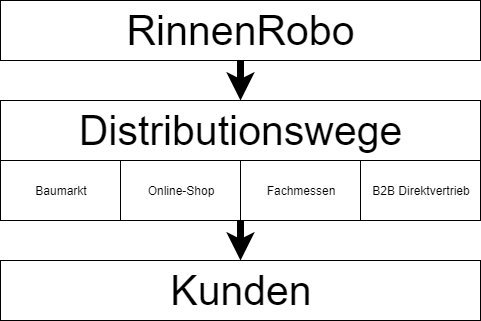
\includegraphics[width = 0.9\textwidth]{Eigene Darstellungen/Distributionswege1.png}

        \caption{Distributionswege (Eigene Dastellung in Anlehnung an Volesungsunterlagen)}
     \end{figure}